\section*{Problema 2.4}

\textbf{Decidimos que dos observaciones $x_i$ , $x_j$ son conectados por una arista en el grafo correspondiente si $x_i$ está entre los k-vecinos más cercanos de $x_i$ o $x_j$ está entre los k-vecinos más cercanos de $x_i$ . Muestra que la adición de una sola observación en este ejemplo puede destruir por completo el desenrollamiento. Márcala en el dibujo y explícalo.}

\begin{figure}[H]
    \centering
    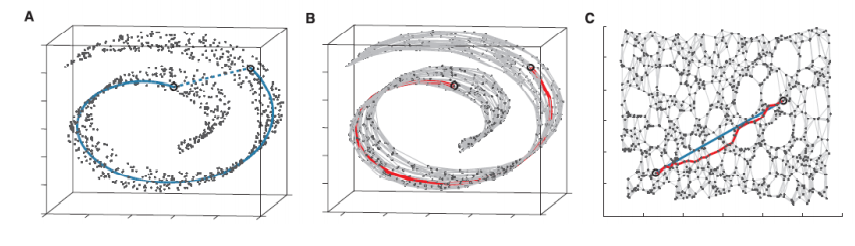
\includegraphics[width=13cm]{Graphics/Problema_2_4.png}
    \caption{}
\end{figure}